\documentclass[a4paper,12pt]{article}

%%% Работа с русским языком
\usepackage{cmap}					% поиск в PDF
\usepackage{mathtext} 				% русские буквы в формулах
\usepackage[T2A]{fontenc}			% кодировка
\usepackage[utf8]{inputenc}			% кодировка исходного текста
\usepackage[english,russian]{babel}	% локализация и переносы
\usepackage{xcolor}
\usepackage{hyperref}
 % Цвета для гиперссылок
\definecolor{linkcolor}{HTML}{799B03} % цвет ссылок
\definecolor{urlcolor}{HTML}{799B03} % цвет гиперссылок

\hypersetup{pdfstartview=FitH,  linkcolor=linkcolor,urlcolor=urlcolor, colorlinks=true}

%%% Дополнительная работа с математикой
\usepackage{amsfonts,amssymb,amsthm,mathtools} % AMS
\usepackage{amsmath}
\usepackage{icomma} % "Умная" запятая: $0,2$ --- число, $0, 2$ --- перечисление

%% Номера формул
%\mathtoolsset{showonlyrefs=true} % Показывать номера только у тех формул, на которые есть \eqref{} в тексте.

%% Шрифты
\usepackage{euscript}	 % Шрифт Евклид
\usepackage{mathrsfs} % Красивый матшрифт

%% Свои команды
\DeclareMathOperator{\sgn}{\mathop{sgn}}

%% Перенос знаков в формулах (по Львовскому)
\newcommand*{\hm}[1]{#1\nobreak\discretionary{}
{\hbox{$\mathsurround=0pt #1$}}{}}
% графика
\usepackage{graphicx}
\graphicspath{{pictures/}}
\DeclareGraphicsExtensions{.pdf,.png,.jpg}
\author{Бурмашев Григорий, БПМИ-208}
\title{Матан, дз -- 9}
\date{\today}
\begin{document}
\maketitle
\section*{Номер 1}
\[
\int_{0}^{2} x^2 dx \int_{x}^{2} \ln(1 + y^2) dy = \int_{0}^{2}  dx \int_{x}^{2} x^2 \ln(1 + y^2) dy \; (=)
\]
Рисуем графичек, внешним интегралом (по иксу) идем от 0 до 2, а внутренним (по y) идем от $x$ до 2, визуально:
\begin{center}
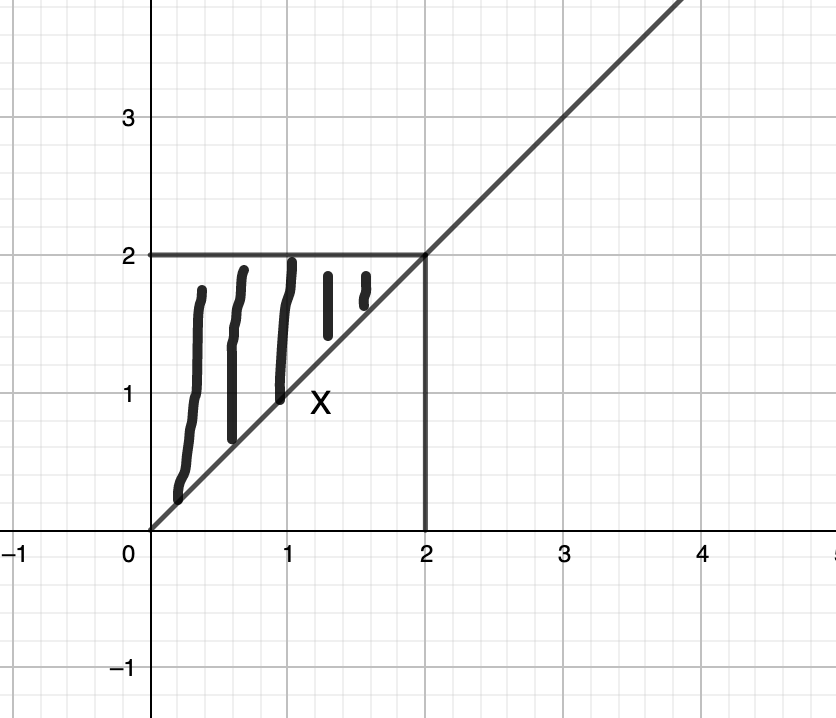
\includegraphics[scale=0.4]{1.png}
\end{center}
Ну теперь собственно "переворачиваем" \; графичек,  меняем порядок интегрирования и считаем:
\[
(=) \int_{0}^{2}  dy \int_{0}^{y} x^2 \ln(1 + y^2) dx  = \int_{0}^{2}  \ln(1 + y^2) \frac{x^3}{3}  \bigg|_0^y dy = 
\]
\[
= \int_{0}^{2}  \ln(1 + y^2) \frac{y^3}{3}  dy = \frac{1}{3} \int_{0}^{2}  \ln(1 + y^2) y^3  dy=
\] 
\[
=\frac{1}{3} \left( \frac{1}{4} y^4 \log (y^2 + 1) \bigg|_0^2 - \frac{1}{4} \int_0^2 \frac{2y^5}{y^2 + 1} dy \right)  = \frac{1}{3} \left(4 \ln 5 - 0 - \frac{1}{2}\int_0^2 \frac{y^5}{y^2 + 1} dy \right) =
\]
\[
=
\frac{1}{3} \left(4 \ln 5 - \frac{1}{4} \int_0^4 \frac{u^2}{u + 1} du \right) = \frac{1}{3} \left(4 \ln 5 - \frac{1}{4} \left(4 + \ln5 \right) \right)  = \frac{1}{3} \left(4 \ln 5 - 1 - \frac{\ln5}{4}\right) =
\]
\[
=\frac{1}{3} \left(\frac{15\ln5}{4} - 1\right) =  \frac{5 \ln 5}{4 } - \frac{1}{3}
\]
\begin{center}
\textbf{Ответ: } 
\[
\int_{0}^{2} x^2 dx \int_{x}^{2} \ln(1 + y^2) dy = \frac{5 \ln 5}{4 } - \frac{1}{3}
\]
\end{center}
\clearpage

\section*{Номер 2}
\[
\iint\limits_D \sgn(x^2 + y^2 -4)dxdy, D = \{(x, y) : x^2 + y^2 \leq 9 \}
\]
По определению функции $\sgn$:
\[
 \sgn(x^2 + y^2 -4) = \begin{cases}
\;1,\;\; x^2 + y^2 > 4 \\
\; 0,\; \;x^2 + y^2 = 4\\
-1 , x^2 + y^2 < 4
\end{cases}
\]
Тогда можно нарисовать графичек:
\begin{center}
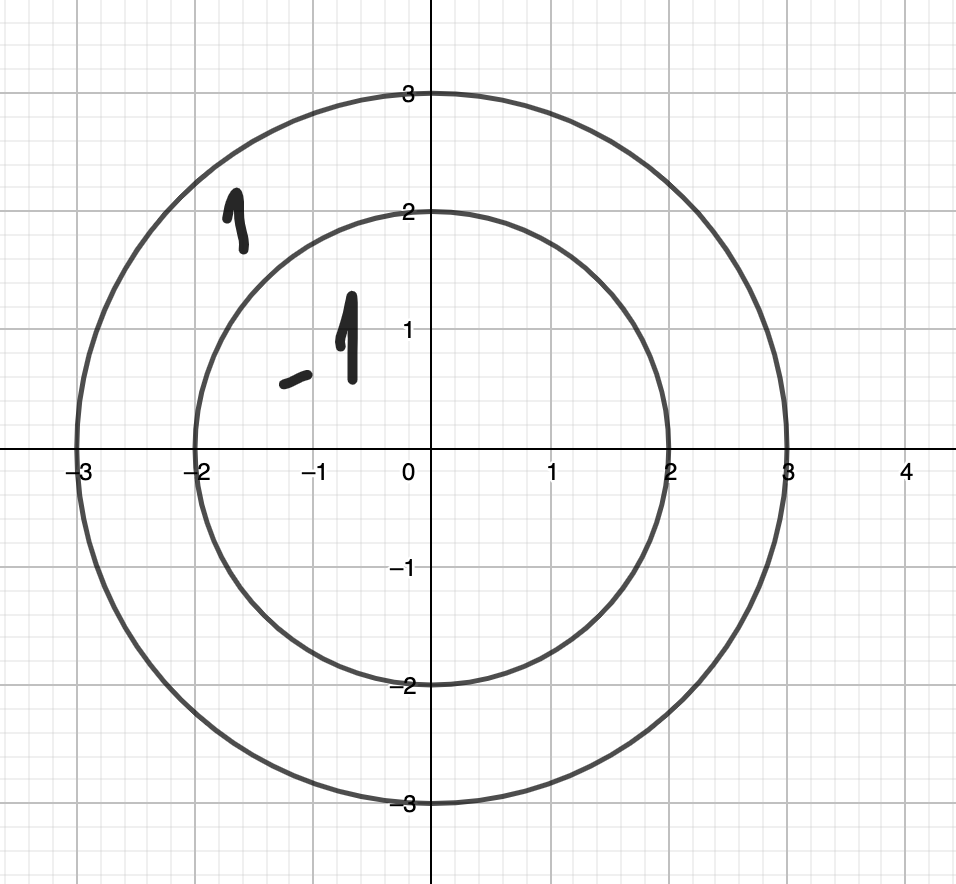
\includegraphics[scale=0.4]{2.png}
\end{center}
Т.е на внутреннем круге радиусом 2 получаем значение функции -1, а на кольце 1. Можем сразу посчитать площади: площадь большого круга с радиусом 3 есть $9 \pi$, площадь маленького круга есть $4 \pi$, тогда площадь кольца $9 \pi - 4pi  = 5\pi$. На точки где функция принимает 0 ($x^2 + y^2 = 4$) забиваем, ибо 0 нас не интересует. Итого:
\[
\iint\limits_{x^2 + y^2 < 4} -1 dx dy + \iint\limits_{4 < x^2 + y^2 < 9} 1 dx dy = -1 \cdot 4\pi +1 \cdot 5 \pi = 5 \pi - 4\pi = \pi
\]
\begin{center}
\textbf{Ответ: } 
\[
\iint\limits_D \sgn(x^2 + y^2 -4)dxdy = \pi
\]
\end{center}
\end{document}
